\documentclass[pdftex]{article}	% the pdftex is essential
\usepackage{xcolor}
\usepackage{pgfplots}
\pgfplotsset{compat=1.13}
\begin{document}
% for documentation see:
%http://www.iro.umontreal.ca/~simardr/pgfplots.pdf


   %\begin{tikzpicture}
	%\begin{loglogaxis}[
		%xlabel={\small number of array emements},
		%ylabel={\small exicution time},
		%legend pos=north west,
		%grid=major,
		%no markers,
		%width=0.66\textwidth,
		%ymax=0.3,
		%]
	    %\addplot
     %[very thick, green!85!black, domain=0:9] table[x index=0, y index=2]
      %{./output.dat} ;
      %\addplot
     %[very thick, blue!85!black, domain=0:9] table[x index=0, y index=1]
      %{./output.dat} ;
      %\addplot
     %[very thick, purple!85!black, domain=0:9] table[x index=0, y index=3]
      %{./output.dat} ;
      %% \addplot
    %%  [very thick, yellow!85!black] table[x index=1, y index=4]
    %%   {./output.dat} ;
      %% \legend{{\small cublas},{\small blas},{\small thrust},{\small local}}
      %\legend{{\small cublas},{\small blas},{\small local}}
	%\end{loglogaxis}
%\end{tikzpicture}
%
%\begin{tikzpicture}
%\begin{semilogxaxis}[
 %xlabel={\small number of array emements},
 %ylabel={\small relative speedup to local},
 %legend pos=north west,
 %grid=major,
 %no markers,
 %width=0.66\textwidth,
 %ymax=30,
 %]
   %\addplot
  %[very thick, blue!85!black, domain=0:9] table[x index=0, y index=1]
   %{./speedup.dat} ;
   %\addplot
  %[very thick, purple!85!black, domain=0:9] table[x index=0, y index=2]
   %{./speedup.dat} ;
   %\legend{{\small blas},{\small cublas}}
%\end{semilogxaxis}
%\end{tikzpicture}
\pgfplotstableread[col sep = comma]{./data/cuWos_data.csv}\mydata
\begin{tikzpicture}
\begin{loglogaxis}[
 xlabel={\small  paths number},
 ylabel={\small relative error},
 legend pos=north east,
 grid=major,
 no markers,
 width=1\textwidth,
 ]
   \addplot
  table[ x index={0}, y index={1}] {\mydata} ;
   \legend{{\small relative error }}
\end{loglogaxis}
\end{tikzpicture}

\begin{tikzpicture}
\begin{semilogxaxis}[
 xlabel={\small current itteration},
 ylabel={\small value},
 legend pos=south east,
 grid=major,
 no markers,
 width=1\textwidth,
 ymax=0.5,
 ymin=0.2,
 xmin=0.1,
 ]
   \addplot
  [very thick, green!85!black, domain=0:9] table[x index={0},y index={2}]
   {\mydata} ;

  \addplot
    [only marks,mark size=1 pt, black] table[x index={0},y index={3}]
    {\mydata} ;

  \legend{{\small expected value},{\small boundary evaluations}}
\end{semilogxaxis}
\end{tikzpicture}

% \pgfplotstableread[col sep = comma]{./data/exit_positions.csv}\exit
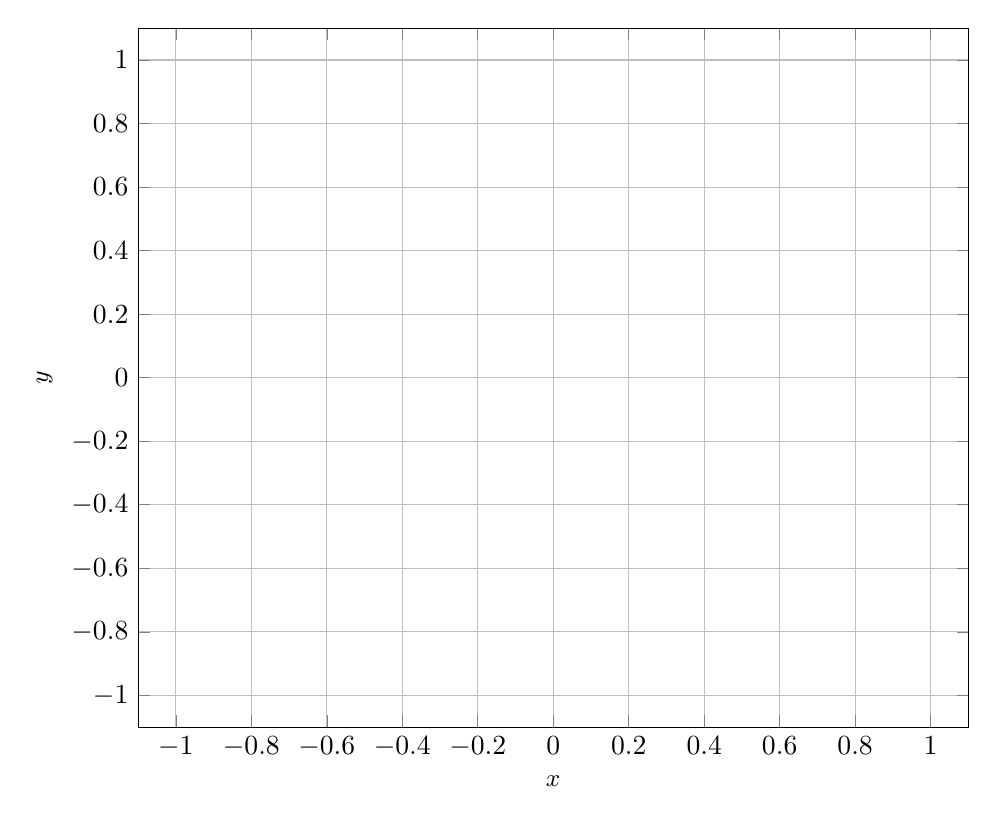
\begin{tikzpicture}
\begin{axis}[
 xlabel={\small $x$},
 ylabel={\small $y$},
 legend pos=north east,
 grid=major,
 width=1\textwidth,
 ymax=1.1,
 ymin=-1.1,
 xmax=1.1,
 xmin=-1.1,
 ]
  %  \addplot
  % [only marks,mark size=1 pt, pink]table[ x index={0}, y index={1}] {\exit} ;
  %  \legend{{\small relative error }}
\end{axis}
\end{tikzpicture}

\end{document}

